% This example is meant to be compiled with lualatex or xelatex
% The theme itself also supports pdflatex
\PassOptionsToPackage{unicode}{hyperref}
\documentclass[aspectratio=1610, 9pt]{beamer}

% Load packages you need here
\usepackage{polyglossia}
\setmainlanguage{german}

\usepackage{csquotes}


\usepackage{amsmath}
\usepackage{amssymb}
\usepackage{mathtools}

\usepackage{hyperref}
\usepackage{bookmark}

% load the theme after all packages

\usetheme[
  showtotalframes, % show total number of frames in the footline
  % dark, % optional dark theme, uncomment to use
]{tudo}

% Put settings here, like
\unimathsetup{
  math-style=ISO,
  bold-style=ISO,
  nabla=upright,
  partial=upright,
  mathrm=sym,
}

\title{Grenzen auf Majoron-Neutrino-Kopplungen aus Supernovaexplosionen in verschiedenen Basen}
\author[J.~Ollesch]{Jonas Ollesch}
\institute[AG Päs]{Arbeitsgruppe Päs \\  Fakultät Physik}
% \titlegraphic{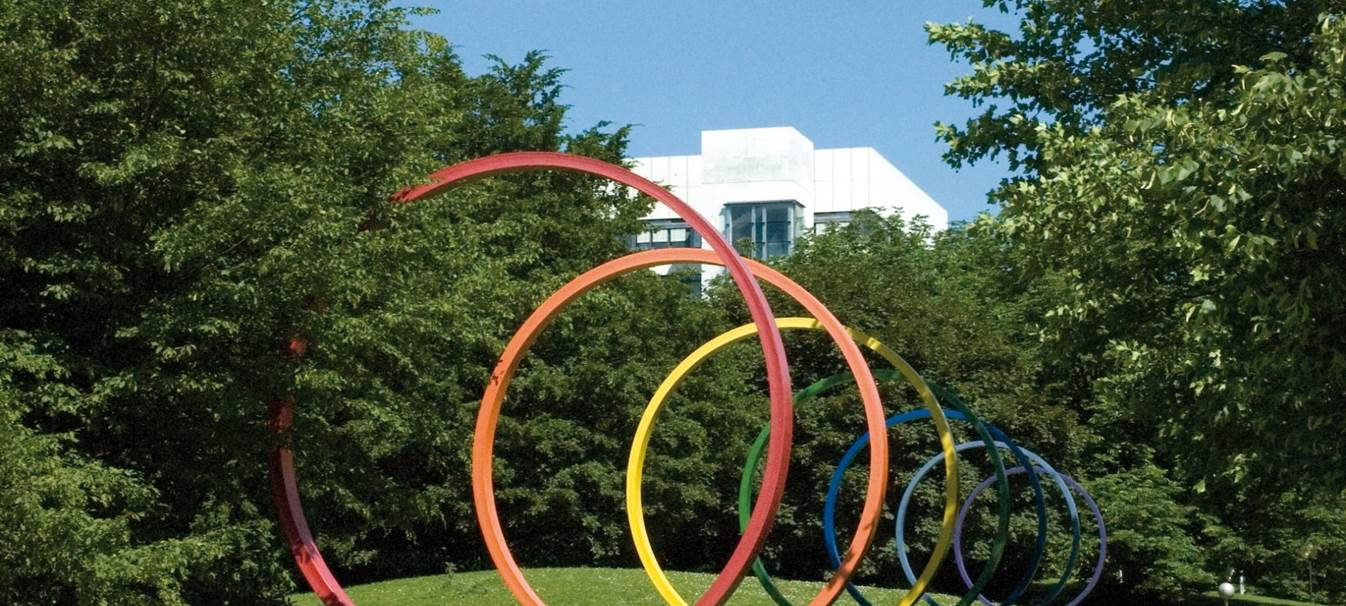
\includegraphics[width=0.7\textwidth]{images/tudo-title-2.jpg}}


\begin{document}

\maketitle

\begin{frame}{Einleitung}
  \begin{itemize}
    \item Nach Standardmodell der Physik sind Neutrinos die einzigen masselosen Fermionen
    \item 2015 erhielten Arthur McDonald und Takaaki Kajita den Nobelpreis für die Entdeckung der Neutrinooszillationen
    Unnötige Kopplungsmatrix
    \begin{equation}
      \tilde{g} = \left( \begin{array}{c c c}
        c^2_{1 2} c^2_{1 3} g_1 + s^2_{12} c^2_{13} \mathrm{e}^{-2 i \delta_1} g_2 + s^2_{13} \mathrm{e}^{-2 i \delta_2}  g_3               &   -s_{12}c_{12}c_{13} g_1 + c_{12} s_{12} c_{13} \mathrm{e}^{-2 i \delta_1} g_2       &   -c^2_{12} s_{13} c_{13} g_1 + s^2_{12} c^2_{13} \mathrm{e}^{-2 i \delta_1} g_2 + s_{13} c_{13} \mathrm{e}^{-2 i \delta_2} g_3  \\ 
        -s_{12}c_{12}c_{13} g_1 + c_{12} s_{12} c_{13} \mathrm{e}^{-2 i \delta_1} g_2                                                       &   s^2_{12} g_1 + c^2_{12} \mathrm{e}^{-2 i \delta_1} g_2                              &   s_{12} c_{12} s_{13} g_1 + s_{12}c_{12}s_{13} \mathrm{e}^{-2 i \delta_1} g_2   \\ 
        -c^2_{12} s_{13} c_{13} g_1 + s^2_{12} c^2_{13} \mathrm{e}^{-2 i \delta_1} g_2 + s_{13} c_{13} \mathrm{e}^{-2 i \delta_2} g_3       &   s_{12} c_{12} s_{13} g_1 + s_{12}c_{12}s_{13} \mathrm{e}^{-2 i \delta_1} g_2        &   c^2_{21} s^2_{13} g_1 + s^2_{12}s^2_{13} \mathrm{e}^{-2 i \delta_1} g_2 + c^2_{13} \mathrm{e}^{-2 i \delta_2} g_3  \\
    \end{array}\right)  
    \end{equation}
      \end{itemize}

  Oneliner zur Installation:\\
  \texttt{\footnotesize\$ cd `kpsewhich --var-value TEXMFHOME` \&\& git clone https://github.com/maxnoe/tudobeamertheme}

  \medskip
  Allgemein zu Beamer und Latex:
  \begin{itemize}
    \item Umfangreicher \LaTeX-Kurs von PeP et Al. \\
      \url{http://toolbox.pep-dortmund.org/notes}
    \item Latex-Beamer Dokumetation:\\
    \url{http://www.ctan.org/pkg/beamer}
  \end{itemize}
\end{frame}

\begin{frame}{Einführung}
  \tableofcontents
\end{frame}

\section{Fonts}
\begin{frame}
  Der Font der im Corporate Design der TU Dortmund vorgesehen ist,
  ist \enquote{Akkurat Office}.

  Falls dieser nicht verfügbar ist, wird als Alternative \enquote{Fira Sans}
  verwendet.

  Für Mathematik wird bei Verwendung von \texttt{xelatex} oder \texttt{lualatex} der Font \enquote{Fira Math} verwendet.
\end{frame}

\begin{frame}{Mathe}
  \begin{align*}
    \nabla \cdot \symbf{B} &= 0 &
    \nabla \cdot \symbf{E} &= \frac{ρ}{ε_0} \\
    \nabla \times \symbf{E} &= -\partial_t \symbf{B} &
    \nabla \times \symbf{B} &= μ_0 \symbf{j} + μ_0 ε_0 \partial_t \symbf{E} &
  \end{align*}
\end{frame}
\end{document}
